\documentclass{beamer-control}
\usepackage{beamer-control-singlefile}
\INCLUDEONLY{Bode’s Relations and Minimum Phase Systems}
\begin{document}
\CONCEPT{Bode’s Relations and Minimum Phase Systems}

\begin{SUMMARY}
\begin{itemize}
\item Minimum phase systems
\item Non-minimum phase systems
\end{itemize}
\vfill References:
\begin{itemize}
\item \astrom{§10.4}
\end{itemize}
\end{SUMMARY}



\SUBCONCEPT{Minimum phase systems}

\begin{frame}{A relation between gain and phase}
\begin{itemize}
\item Bode plots often seem to depict a correlation between the gain and phase curves of a system
\item For a special class of systems there is an explicit relation
\item  For minimum phase systems, systems that do not have time delays or poles and zeros in the right half-plane and have $\tfrac{\log G(s)}{s}\rightarrow 0$ as $s\rightarrow \infty$, then the phase is uniquely given by the shape of the gain curve
\item These systems are called minimum phase as they have the smallest phase lag of all systems with the same gain curve
\end{itemize}
\end{frame}


\begin{frame}{Phase from gain}
\begin{itemize}
\item For minimum phase systems, the phase is given by
\begin{align*}
\operatorname{arg}G(i\omega_0) &= \frac{\pi}{2}\int^\infty_0 f(\omega) \frac{\mathrm{d}\log |G(i\omega)|}{\mathrm{d}\log \omega} \frac{\mathrm{d}\omega}{\omega}\\
&\approx
\left. \frac{\pi}{2}\frac{\mathrm{d}\log |G(i\omega)|}{\mathrm{d}\log \omega}\right|_{\omega=\omega_0}
\end{align*}
where $f$ is the weighting kernel $f(\omega)=\frac{2}{\pi^2} \log \left|\frac{\omega+\omega_0}{\omega-\omega_0}\right|$ with $\int^\infty_0 f(\omega)\frac{\mathrm{d}\omega}{\omega}=1$
\item Basically, the phase curve for minimum phase systems is a weighted average of the derivative of the gain curve
\end{itemize}
\end{frame}

\begin{frame}{Example}
\begin{itemize}
	\item Consider the system with transfer function 
	\[G(s)=s^n\]
	\item We have $\log G(s) = n\log s$ and hence $\tfrac{\mathrm{d}\log G(s)}{\mathrm{d} \log s}=n$ so
	\[\operatorname{arg}G(i\omega_0) = \frac{\pi}{2}\int^\infty_0 f(\omega) \frac{\mathrm{d}\log |G(i\omega)|}{\mathrm{d}\log \omega} \frac{\mathrm{d}\omega}{\omega}=n\frac{\pi}{2}\int^\infty_0 f(\omega)  \frac{\mathrm{d}\omega}{\omega}\]
	\[\operatorname{arg}G(i\omega_0) = n\frac{\pi}{2}\]
	\item Therefore, if the gain curve has a constant slope $n$, the phase curve is a horizontal line $\operatorname{arg}G(i\omega)=\tfrac{n\pi}{2}$
\end{itemize}
\end{frame}

\SUBCONCEPT{Non-minimum phase systems}

\begin{frame}{When Bode's relation doesn't hold}
\begin{itemize}
\item Non-minimum phase systems are quite common in the real world and possess either time delays, right half-plane zeros, or right half-plane poles
\item In these systems, the phase isn't uniquely defined from the gain curve
\item We can illustrate how these effects influence the phase curve of our system by comparing transfer functions that have the same gain curve

\end{itemize}
\end{frame}

\begin{frame}{Example}
\begin{itemize}
	\item The transfer function $G(s)=\frac{a-s}{a+s}$ with $a>0$ has a zero $s=a$ in the right half-plane, with unit gain $|G(i\omega)|=1$ and phase curve given by $\operatorname{arg} G(i\omega) = -2\arctan (\tfrac{\omega}{a})$
	\item The transfer function $G(s)=\frac{s+a}{s-a}$ with $a>0$ has a pole in the right half-plane, has unit gain $|G(i\omega)|=1$ and phase  $\operatorname{arg} G(i\omega) = -2\arctan (\tfrac{\omega}{a})$
	\item The corresponding minimum phase system is the transfer function $G(s)=1$
\end{itemize}
\end{frame}

\begin{frame}{Example continued}
In the below plots, the phase curve of the corresponding minimum phase system with transfer function $G(s)=1$ is shown as dashed lines
\begin{figure}
	\centering
	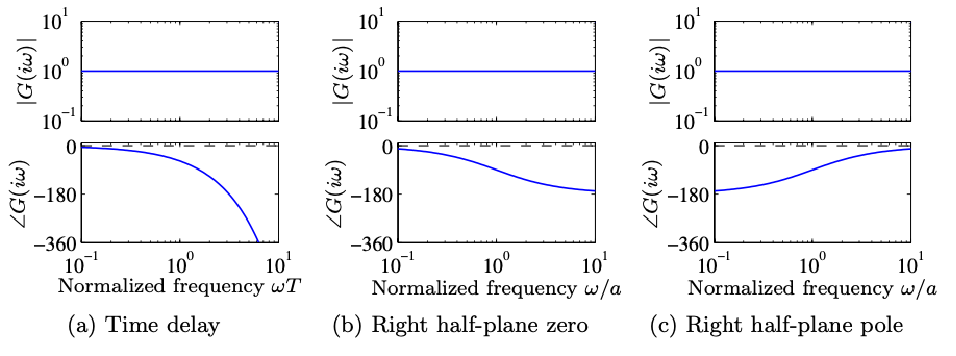
\includegraphics[width=0.9\linewidth]{figure10.15}
	\\
	\textbf{Figure 10.15:} Bode plots of non-minimum phase systems. (a) Time delay $G(s)=e^{-sT}$, (b) RHP zero $G(s)=\frac{a-s}{a+s}$, (c) RHP pole $G(s)=\frac{s+a}{s-a}$. 
\end{figure}
\end{frame}

\SUMMARYFRAME
\FINALE

\end{document}
